%%%%%%%%%%%%%%%%%%%%%%%%%%%%%%%%%%%%%%%%%
% Simple Sectioned Essay Template
% LaTeX Template
%
% This template has been downloaded from:
% http://www.latextemplates.com
%
% Note:
% The \lipsum[#] commands throughout this template generate dummy text
% to fill the template out. These commands should all be removed when 
% writing essay content.
%
%%%%%%%%%%%%%%%%%%%%%%%%%%%%%%%%%%%%%%%%%

%----------------------------------------------------------------------------------------
%	PACKAGES AND OTHER DOCUMENT CONFIGURATIONS
%----------------------------------------------------------------------------------------

\documentclass[12pt]{article} % Default font size is 12pt, it can be changed here


\usepackage{polski}
\usepackage[utf8]{inputenc}

\usepackage{geometry} % Required to change the page size to A4
\geometry{a4paper} % Set the page size to be A4 as opposed to the default US Letter
\newgeometry{tmargin=2cm, bmargin=2cm, lmargin=2cm, rmargin=2cm}

\usepackage{graphicx} % Required for including pictures

\usepackage{float} % Allows putting an [H] in \begin{figure} to specify the exact location of the figure
\usepackage{wrapfig} % Allows in-line images such as the example fish picture

\usepackage{lipsum} % Used for inserting dummy 'Lorem ipsum' text into the template

\linespread{1.2} % Line spacing

%\setlength\parindent{0pt} % Uncomment to remove all indentation from paragraphs

\graphicspath{{Pictures/}} % Specifies the directory where pictures are stored

\begin{document}

%----------------------------------------------------------------------------------------
%	TITLE PAGE
%----------------------------------------------------------------------------------------

\begin{titlepage}

\newcommand{\HRule}{\rule{\linewidth}{0.5mm}} % Defines a new command for the horizontal lines, change thickness here

\center % Center everything on the page

\textsc{\LARGE Politechnika Wrocławska}\\[1.5cm] % Name of your university/college
\textsc{\Large Projekt usług multimedialnych}\\[0.5cm] % Major heading such as course name
\textsc{\large Kod kursu: TLEU00103P, Termin: Piątek, 7:30-9:00 TP}\\[0.5cm] % Minor heading such as course title

\HRule \\[0.4cm]
{ \huge \bfseries Projekt systemu sensorycznego dla energooszczędnego, inteligentnego mieszkania jednorodzinnego}\\[0.4cm] % Title of your document
\HRule \\[1.5cm]

\begin{minipage}{0.4\textwidth}
\begin{flushleft} \large
\emph{Autorzy:}\\
inż. Łukasz \textsc{Joksch}(200963) \\
inż. Tomasz \textsc{Kowalik}(200943) \\
inż. Piotr \textsc{Tazbir}(201029)
\end{flushleft}
\end{minipage}
~
\begin{minipage}{0.4\textwidth}
\begin{flushright} \large
\emph{Opiekun:} \\
dr Piotr \textsc{Piotrowski} % Supervisor's Name
\end{flushright}
\end{minipage}\\[4cm]

{\large \today}\\[3cm] % Date, change the \today to a set date if you want to be precise

%\includegraphics{Logo}\\[1cm] % Include a department/university logo - this will require the graphicx package

\vfill % Fill the rest of the page with whitespace

\end{titlepage}



\newpage % Begins the essay on a new page instead of on the same page as the table of contents 

%----------------------------------------------------------------------------------------
%	INTRODUCTION
%----------------------------------------------------------------------------------------

\section{Wstęp} 

Niniejszy projekt ma za zadanie pokazać nowoczesne podejście w projektowaniu systemu sensorycznego, który pomoże zaoszczędzić takie zasoby jak energia elektryczna, prąd, ogólnie rozumiane ogrzewanie. Czyni to gospodarstwo domowe ekologicznym, wygodnym ale co ważniejsze - właściciele zaoszczędzą pieniądze nie marnując tych zasobów. Celem projektu jest takie dobranie komponentów, by zapotrzebowanie na prąd było jak najmniejsze, jednak, by jego minimalny pobór nie wpływał negatywnie na jakość życia w takim mieszkaniu. Jest to możliwe dzięki zastosowaniu najnowszych technologii mikroprocesorowych,sprzętu sterującemu poszczególnymi elementami systemu oraz dzięki stworzeniu optymalnego oprogramowania i algorytmów zarządzających.
\\ \\
W tym projekcie pragniemy podkreślić szczególne znaczenie kolejnych modułów w kontekście konkretnych oszczędności, tj. będziemy chcieli pokazać jak dany element przyczynia się do powstania oszczędności. W miarę możliwości, na ogólnym poziomie koncepcyjnym przedstawione zostaną sposoby magazynowania zasobów, tak by uniknąć ich marnowania. 

\section{Założenia projektowe i wykorzystane technologie}
Głównym założeniem projektowym jest stworzenie takiego systemu, który będzie przyjazny użytkownikowi, tj. jego istnienie będzie wspierało domowników - uczyni życie wygodniejszym. Pragniemy uniknąć sytuacji, w której takie rozwiązanie utrudniałoby korzystanie z mieszkania lub było uciążliwym. Wszystkie przedsięwzięcia będą zmierzały do tego by zminimalizować koszty utrzymania gospodarstwa domowego, optymalizując tym samym wykorzystanie zasobów.

\subsection{Zastosowane technologie}
Kolejne podsystemy rozwiązania charakteryzują się strukturę modularną, tzn. że są całkowicie wymienialne. Ważniejszym jest jednak fakt, iż takie podejście czyni projekt w pełni skalowalnym. Wszystkie zespoły modułów podlegają centralnemu serwerowi, pełniącemu rolę centrali zarządzającej. Centrala ta to mikrokomputer RaspberryPI 3. Zdecydowano się na jego wykorzystanie względu na niskie napięcie zasilania - 5V oraz minimalny pobór prądu - ok. 300mA. Pozwoli to na długą i niezakłóconą pracę systemu na zasilaniu bateryjnym. Należy podkreślić, iż zastosowano turbinę wiatrową i panele słoneczne do wytwarzania energii elektrycznej. Takie podejście umożliwia wykorzystania naturalnych zasobów i znacząco ograniczyć koszty eksploatacji domu.
\\ \\
Główną zaletą proponowanego rozwiązania jest bezprzewodowa łączność pomiędzy modułami, dzięki zastosowaniu transceiver'ów WiFi. Implementacja takich urządzeń powoduje, iż nie jest koniecznym prowadzenie dodatkowego okablowania komunikacyjnego - oszczędzamy w ten sposób pieniądze dzięki braku konieczności zakupu przewodów. Dodatkowo nie jest wymagany remont mieszkania, czy też ingerencja w jego architekturę. Porzucono pomysł komunikacji przez bluetooth, ze względu na mniejszy dystans zasięgu oraz mniejsze możliwości konfiguracyjne.
Ponadto zastosowanie technologii WiFi pozwoli na łatwą i szybką diagnostykę działania takich modułów.
\\ \\ 
W nawiązaniu do centrali zarządzającej, użytkownik będzie miał możliwość łatwą administracją systemu dzięki panelom administracyjnym. W zależności od potrzeb danego klienta jest możliwość zastosowania dowolnej liczby paneli na terenie całego gospodarstwa domowego. Tą rolę będą pełniły tablety z dedykowaną aplikacją mobilną, która będzie prezentowała wskaźniki przewidziane w projekcie (aktualna temperatura w pomieszczeniach, sygnalizacja włączonego oświetlenia, sygnalizacja obecności domowników etc.). Dodatkowo,jeżeli klient wyrazi taką wolę, możliwa będzie instalacja identycznej aplikacji na jego smartfonie, tak by mógł zarządzać swoim mieszkaniem zdalnie.

\section{Zarządzanie energią elektryczną}
W tym rozdziale zostaną scenariusze działań podejmowanych przez system w celu niemarnotrawienia prądu. Działania te dotyczyć będą oświetlenia, wykrywania zdarzeń polegających na pozostawieniu włączonego urządzenia elektrycznego, podczas nieobecności lokatora czy regulowanie naturalnego oświetlenia w zależności od pory dnia.

\subsection{Zastosowane podejście sprzętowe}
Chcąc mieć możliwość elektronicznego sterowania oświetleniem, czy też gniazdami elektrycznymi, które są systemami elektrycznymi - należy stworzyć interfejs ze sterującą nimi elektroniką. Możliwe to jest dzięki zastosowaniu modułów przełączników opartych na triakach i optotriakach. Te moduły to elektroniczne wyłączniki, których zadaniem jest załączanie lub rozłączanie przewodu zasilającego. W ogólnym uproszczeniu ich zasada działania polega na sterowaniu linią zasilania o dużym napięciu, przewodzącej duży prąd (~230V, >1A), małym napięciem i małym prądem (3,3V DC, <20mA). Ponadto stosując takie podejście, w odróżnieniu od modułów przełączników opartych na przekaźnikach elektromagnetycznych, zachowujemy izolację optyczną między instalacją elektryczną i elektroniczną. W przypadku awarii układu, najczęściej nie jest konieczna wymiana całego modułu, lecz, np. samego optotriaka.

\subsection{Zarządzanie oświetleniem}
Użytkownik systemu ma możliwość, w każdej chwili, sprawdzenia czy w danym pomieszczeniu włączone jest oświetlenie i jeżeli będzie widział konieczność, może je wyłączyć w dowolnej części mieszkania. Jest to przedstawione w dalszej części opracowania.
\subsubsection{Czujnik zmierzchu}
Na zewnątrz budynku zainstalowano czujnik zmierzchu, który pokazuje procentową wartość nasłonecznienia. Użytkownik, może uzależnić od tego parametru scenariusze zarządzania energią elektryczną. Na szczególną uwagę zasługuje sposobność ustawienia zależności, w której to gdy nastanie ranek oświetlenie zewnętrze mieszkania czy wybranych pomieszczeń zostanie wyłączone. W rezultacie pomieszczenia będą oświetlane światłem naturalnym. Oczywiście, należy nadmienić, że wyższy priorytet będzie miało ustawienie ręczne, tj. takie przez włączenie wewnątrz budynku oświetlenia w danym pokoju celowo przed mieszkańca(włącznikiem tradycyjnym lub z panelu - tabletu).

\subsubsection{Definiowane okna czasowe}
Dodatkową funkcjonalnością jest możliwość zdefiniowania harmonogramu uruchomienia oświetlenia (oraz wyłączenia) dla każdego punktu oświetleniowego. Dzięki temu będzie można ustawić przez jaki okres czasu ma być uruchomione oświetlenie zewnętrzne czy oświetlenie klinkierowe korytarzy. Przewiduje się bowiem, iż użytkownik chce mieć możliwość odgórnego zadeklarowania godzin pracy oświetlenia z pominięciem czujnika zmierzchu, np. w sytuacji nie chce mieć uruchomionego oświetlenia zewnętrznego przez całą noc a wyłącznie przez godzinę od chwili gdy nastanie zmrok, i np. na godzinę przed świtem.

\subsubsection{Zarządzanie gniazdami elektrycznymi}
Funkcjonalność opisywana poniżej jest opcjonalną i dla każdego pomieszczenia może zostać wyłączona (później w dowolnej chwili można ją włączyć) Ta funkcjonalność ma podwójne zastosowanie. Z jednej strony pozwala zaoszczędzić pieniądze wyłączając nieużywane urządzenia,  drugiej strony pełni rolę prewencyjną chroniącą przed przegrzaniem się sprzętu, a w skrajnych przypadkach przed ich spaleniem.
\\
W każdym gniazdku zainstalowano moduł watomierza.Dzięki temu możliwy będzie badanie poboru prądu w danej chwili. Pozwoli na reagowanie systemu w momencie zauważenia, że przez długi czas jest znaczny pobór - na tablecie pojawi się dobrze widoczny alert. System jest w stanie wykryć obecność osób w pomieszczeniach przy pomocy czujników ruchu. Pozwoli to oszczędzać energię elektryczną w taki sposób, iż gdy system ie wykryje obecności człowieka w pokoju, a stwierdzi zwiększony pobór z gniazdka, wyłączy je. Chcąc uniknąć sytuacji, w której system wyłączy specjalnie pozostawione przez użytkownika urządzenie, np. ładowarkę podczas ładowania telefonu - użytkownik będzie mógł zasygnalizować taką konieczność na tablecie sterującym systemem. Rozwiązane to zostanie za pomocą przycisku blokady automatycznego wyłączenia prądu.
\\
Ponadto, w rozwiązaniu zaimplementowano oddzielne reguły dla urządzeń potencjalnie niebezpiecznych, takich których pozostawienie uruchomionych bez nadzoru człowieka może przyczynić się, np. do pożaru. Dla wszystkich urządzeń, dla których prąd pracy wynosi powyżej 2A, są uruchomione, a w pomieszczeniu nie zostanie wykryty użytkownik - gniazdko, z którego jest zasilane zostanie odłączone od energii elektrycznej.



\section{Zarządzanie zasobami wody}
Sensory tego obszaru wykrywać będą zdarzenie polegające na pozostawieniu otwartych zaworów, kranów w chwili nieobecności domownika. 
\\
Rozwiązanie to ma na celu wspomóc racjonale gospodarowanie wody w gospodarstwie domowym. We wszystkich kranach zostaną zamontowane zawory wodne z czujnikiem ruchu i odległości. Przepływ strumienia wody będzie możliwy wyłącznie gdy w obszarze zlewu(zakres widoczności czujników) pojawi się jakiś obiekt, np. ręce, naczynia. Jednocześnie krany będą miały przełączniki pozwalające podtrzymać strumień wody przez dłuższy czas. Unikniemy dzięki temu sytuacji, w której zawory kranu zostaną niezakręcone.

\section{Zarządzanie ogrzewaniem mieszkania}
Chcąc zapewnić możliwie najbardziej ekologiczne, a zarazem ekonomiczne rozwiązanie ogrzewania domu - zastosowano ogrzewanie gazem ziemnym. Piec grzewczy posiada dedykowany, dostarczany przez producenta, komputer sterujący nim. Jednak chcąc zapewnić integralność całego systemu - zostanie on podłączony interfejsem API do centrali RaspberryPI. Takie rozwiązanie pozwoli przenieś funkcje wspomnianego sterownika do naszego serwera,co umożliwi sterowanie nim z poziomu dostarczanego przez nas oprogramowania. Rozwiązanie zapewnia możliwość ustawiania okien czasowych, w których piec powinien (lub nie) pracować. Ponadto, dzięki zastosowaniu czujników temperatury i regulatorów zaworów na kaloryferach - użytkownik będzie miał możliwość zdefiniowania jaką temperaturę chce uzyskać w pokoju. Zastosowawszy termometry elektroniczne, w dokładny sposób  można określić aktualną temperaturę w pomieszczeniu i na tej podstawie system określi czy występuje konieczność uruchomienia pieca grzewczego i w konsekwencji doregulowania kaloryferów. Chcąc maksymalnie zoptymalizować rozwiązanie, system jest w stanie poinformować użytkowników


\section{System alarmowy}
W ramach projektu systemu sensorycznego przemyśliwujemy powstanie podstawowej wersji systemu alarmowego, który w zadanym oknie czasowym lub na żądanie uzbroi się i będzie ostrzegał o potencjalnym zagrożeniu wynikającym z niepożądanej próby przedostania się intruza na teren posesji. Ze względu na złożoność i wielopoziomowość zagadnienia, zostały zaimplementowane następujące funkcje:
\begin{enumerate}
\item 
wykrycie ruchu przez czujniki podczernieni;
\item 
Wykrycie otwarcia drzwi lub okien;
\item 
sygnalizacja dźwiękowo-akustyczna;
\item 
powiadomienie odpowiednich służb prewencji;
\item 
powiadomienie o zajściu właścicieli mieszania drogą poczty elektronicznej oraz poprzez wiadomość SMS.
\end{enumerate}

\section{Prezentacja danych i zarządzanie systemem}
Rozdział ten przedstawia podsumowanie całego projektu. Prezentujemy tu relacje między poszczególnymi elementami projektu. Chcąc pokazać ideę funkcjonowania projektu poniżej przedstawiono na diagramie:
\begin{figure}[!h]
  \centering
  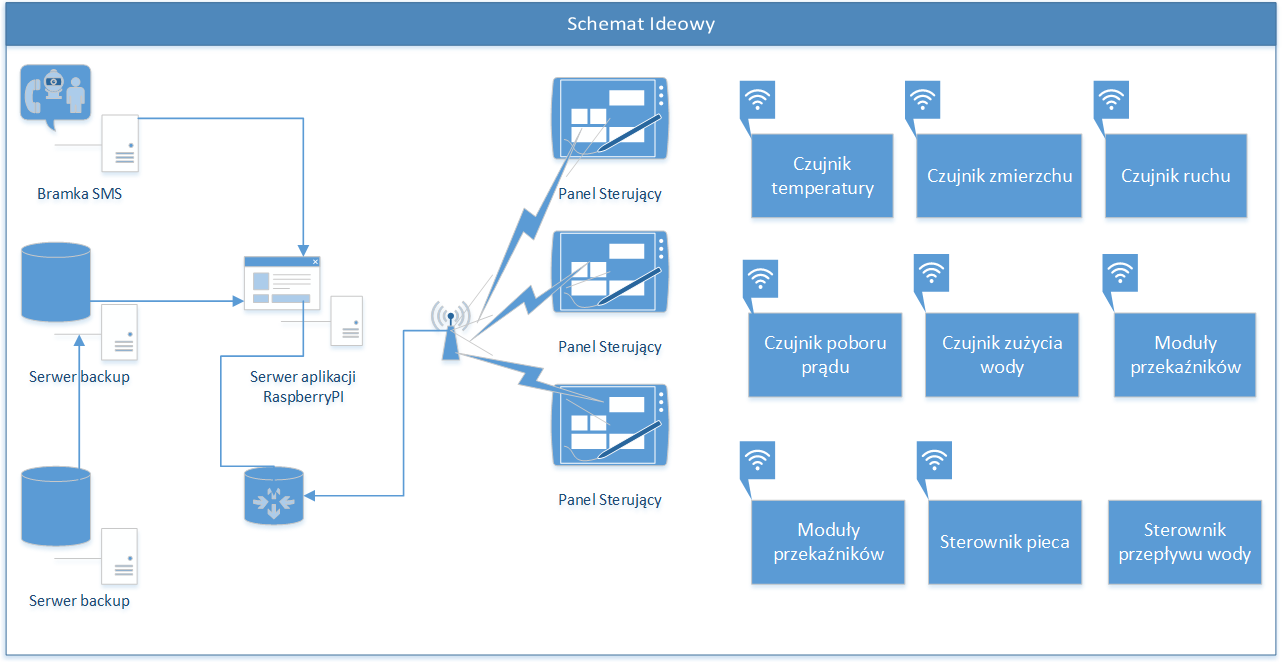
\includegraphics[width=\columnwidth]{images/Rysunek1.png}
  \caption{Diagram ideowy}
\end{figure}

\subsection{Wykorzystane technologie}
\begin{itemize}
\item RaspberryPI 3
\item Moduł GSM/GPRS G510
\item Moduł WiFi WM-G-MR-09 Marvell8686 
\item Czujnik temperatury DS18B20
\item Czujnik zmierzchowy HL470
\item Czujnik ruchu ALER MINI-W
\item Bateria Umywalkowa Bezdotykowa Sensor Fotokomórka Foton
\end{itemize}

\subsection{Scenariusz 1. - Sterowanie oświetleniem}
Ten scenariusz przedstawia model przepływu danych w systemie związanych z zarządzaniem oświetleniem.
\begin{enumerate}
\item 
W systemie zdefiniowano następujące parametry domyślne:
	\begin{itemize}
	\item 
	Oświetlenie zewnętrzne włącza się, gdy poziom 	nasłonecznienia spadnie poniżej 30\%
	\item 
	Oświetlenie zewnętrzne wyłącza się po godzinie 1:00
	\item 
	Oświetlenie wewnętrzne (dla każdego z pomieszczeń mieszkalnych) wyłącza się, gdy danym pokoju nie odnotowano obecności domownika (określane na podstawie czujnika ruchu) w przeciągu ostatnich 20 minut;
	\item
	Na ekranie sterującym istnieje możliwość wyłączenia sprawdzania obecności użytkownika - wówczas to domownik decyduje o momencie wyłączenia świetlenia;
	\item 
	Oświetlenie wewnętrzne (dla każdego z pomieszczeń) zostaje wyłączone o godzinie 1:00, o ile mieszkaniec nie wyłączył te opcji na panelu użytkownika;
	\item 
		Oświetlenie łazienek i toalet wyłącza się, gdy danym pokoju nie odnotowano obecności domownika (określane na podstawie czujnika ruchu) w przeciągu ostatnich 5 minut;
	\item 
	Oświetlenie garażu, piwnicy i strychu wyłącza się, gdy danym pokoju nie odnotowano obecności domownika (określane na podstawie czujnika ruchu) w przeciągu ostatnich 10 minut;.
	\end{itemize}

\item
Sterowanie każdym modułem oświetlenia jest możliwe z poziomu panelu użytkownika oraz przez tradycyjny wyłącznik podtynkowy;
\item 
Możliwym jest zmiana poszczególnych zmiennych, będących parametrami, o których mowa punkcie 1. Scenariusza 1.;
\item 
Dopuszcza się możliwość blokowania funkcji sprawdzania obecności domowników w zadanych interwałach czasowych.

\end{enumerate}

\newpage
\section{Demonstracja przykładowego dashboard'u}
W tym miejscu zostaną dodane zrzuty ekranowe dashboardów w momencie ich ukończenia.

\begin{figure}[!h]
  \centering
  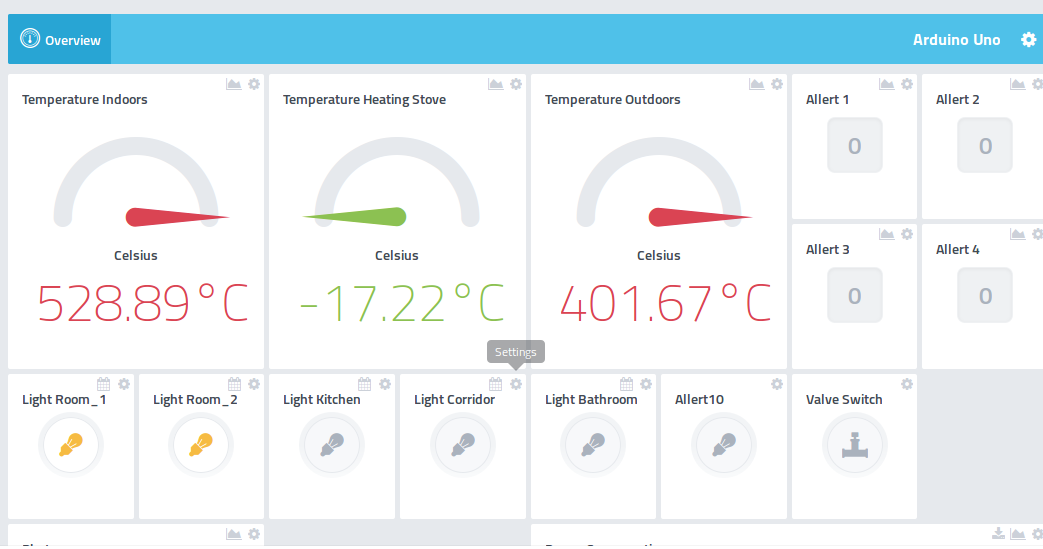
\includegraphics[width=\columnwidth]{images/1.png}
  \caption{Wskaźniki}
\end{figure}

Na rysunku 2.  przedstawiono działanie systemu, można zauważyć włączone swiatła w pokojach oraz temperaturę w domu, na zewnątrz oraz temperaturę kotła CO. Temperatura nie jest wyznacznikiem rzeczywistej temperatury ze względu na elementy użyte do symulacji.

\begin{figure}[!h]
  \centering
  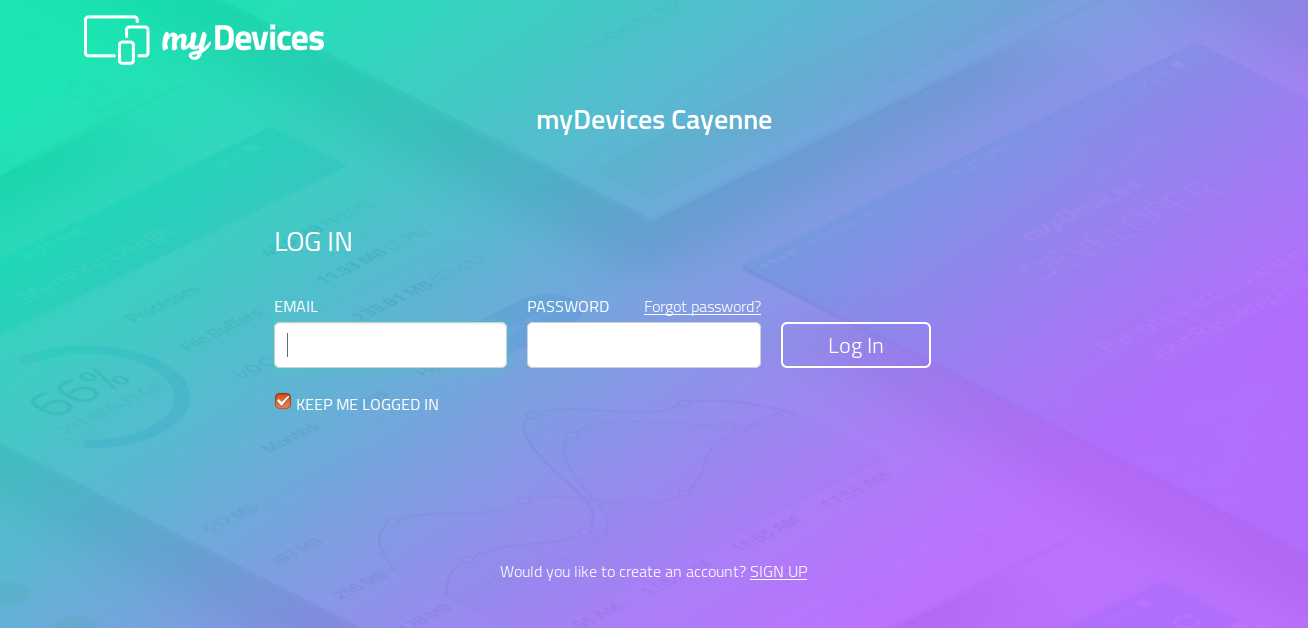
\includegraphics[width=\columnwidth]{images/2.png}
  \caption{Logowanie}
\end{figure}
Na samym początku (odniesienie do rysunku 3.), aby skorzystać z systemu Cayenne do stworzenia oraz zarządzania systemem sensorycznym inteligentnego budynku trzeba się zalogować do myDevices Cayeene. Udostępni nam to szeroki wachlarz rozwiązań oraz urządzeń kompatybilnych z systemem które mogą być wykorzystane dla naszych potrzeb. Istnieje również możliwość zdefiniowania własnego urządzenia.

\begin{figure}[!h]
  \centering
  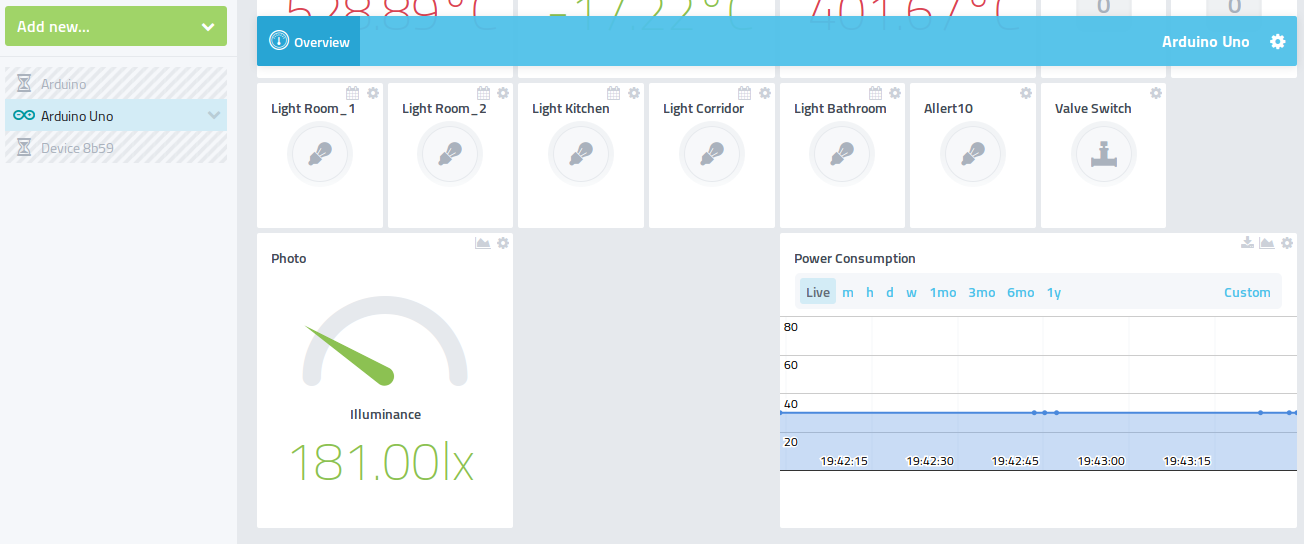
\includegraphics[width=\columnwidth]{images/3.png}
  \caption{Pobór prądu}
\end{figure}

Rysunek 4. ten przedstawia pobór prądu w czasie rzeczywistym a także nasłonecznienie w naszym mieszkaniu od którego zależne mogą być rolety okienne, czy światła w pokojach.

\begin{figure}[!h]
  \centering
  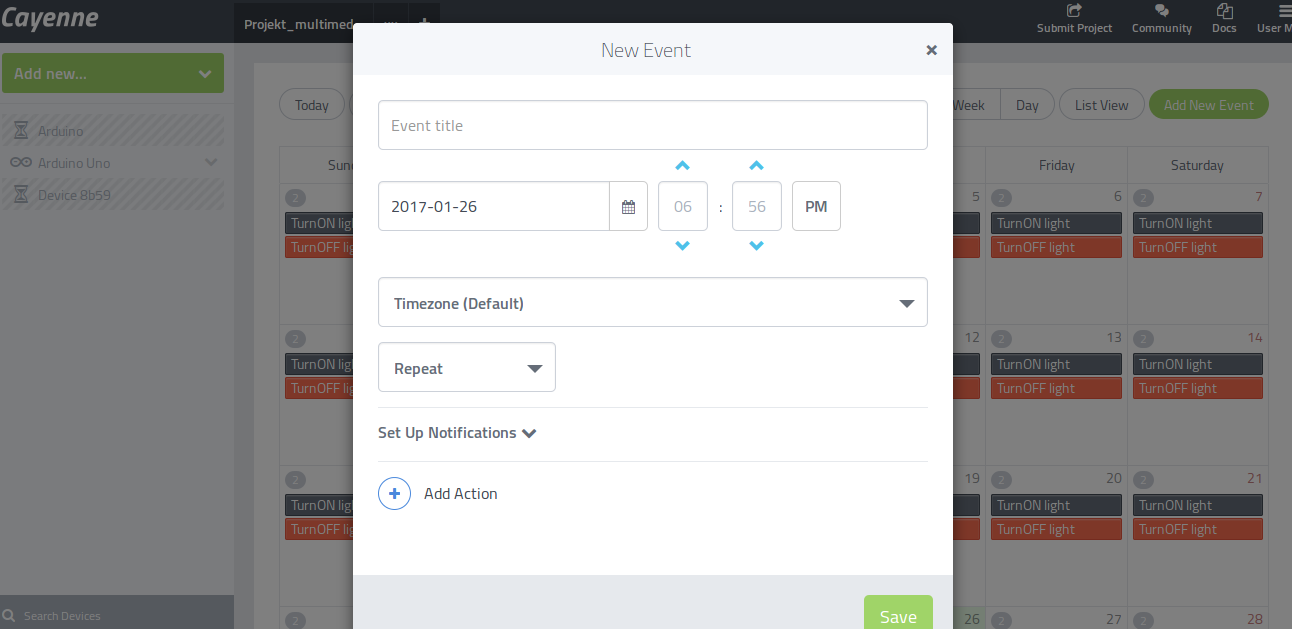
\includegraphics[width=\columnwidth]{images/4.png}
  \caption{Zarządzanie}
  \end{figure}

Na tym rysunku 5. przedstawiono w jaki sposób można zarządzać i tworzyć akcje tj. gaszenie świateł i ich zapalanie o określonych godzinach w całym domu lub jego cześci (np. pokoju) a także wiele innych.

\begin{figure}[!h]
  \centering
  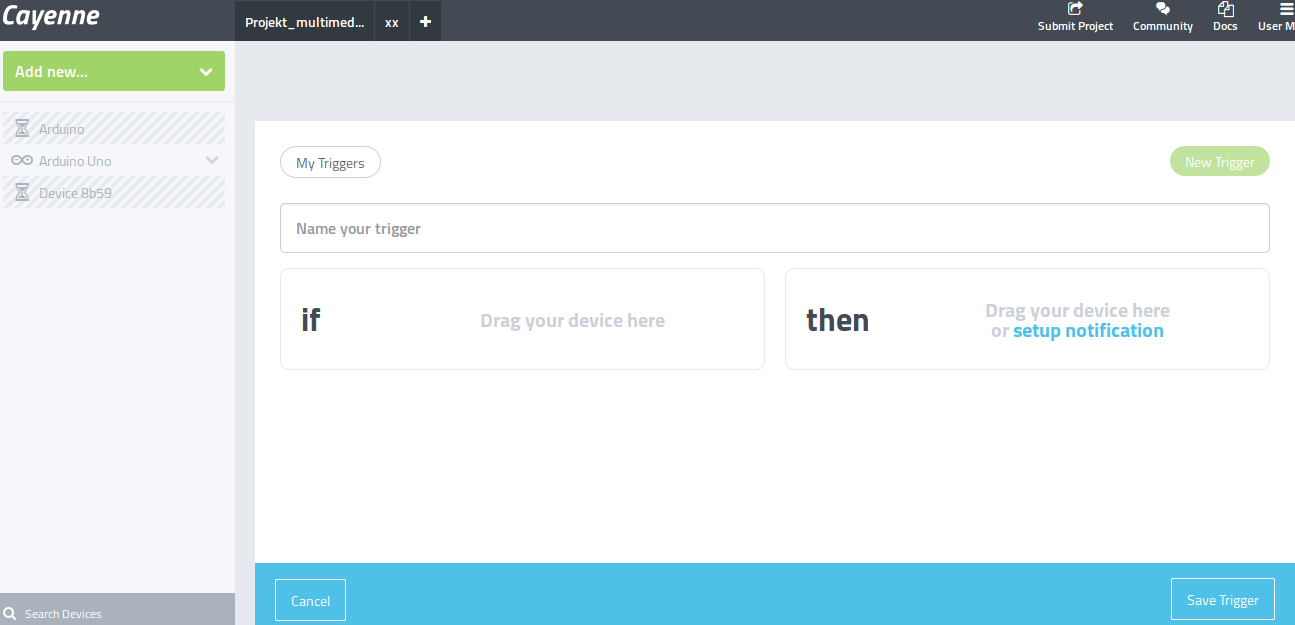
\includegraphics[width=\columnwidth]{images/5.png}
  \caption{Warunki}
\end{figure}
Rysunek 6. przedstawia w jaki sposób można utworzyć znane z tekstowych języków programowania instrukcje warunkowe (if...else) czyli co ma być następstwem jakiegoś zdarzenia.

\begin{figure}[!h]
  \centering
  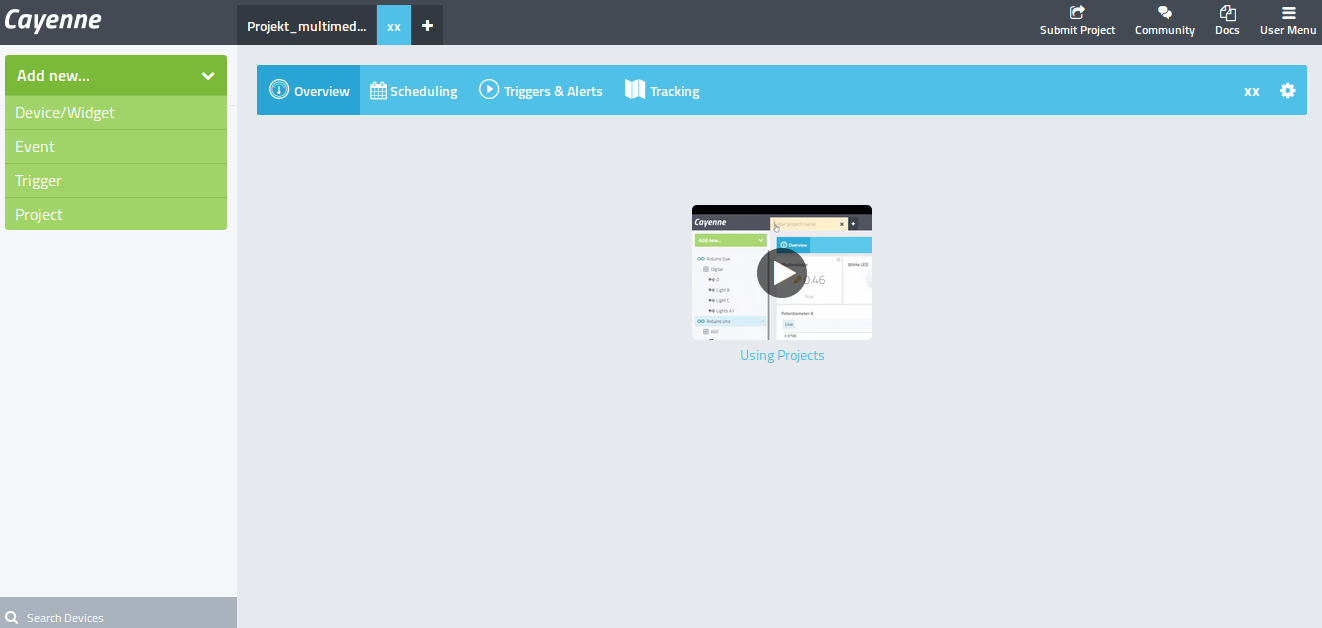
\includegraphics[width=\columnwidth]{images/6.png}
  \caption{Modularność}
\end{figure}
Rysunek 7. przedstawia ekran po zalogowaniu do swojego myDevices Cayeene. Zwrócić można uwagę na zieloną liste w górnym lewym rogu są tam odpowiednie opcje jak stworzenie nowego projektu czy wyranie urządzenia którym chcemy sterować (Device/Widget).

\begin{figure}[!h]
  \centering
  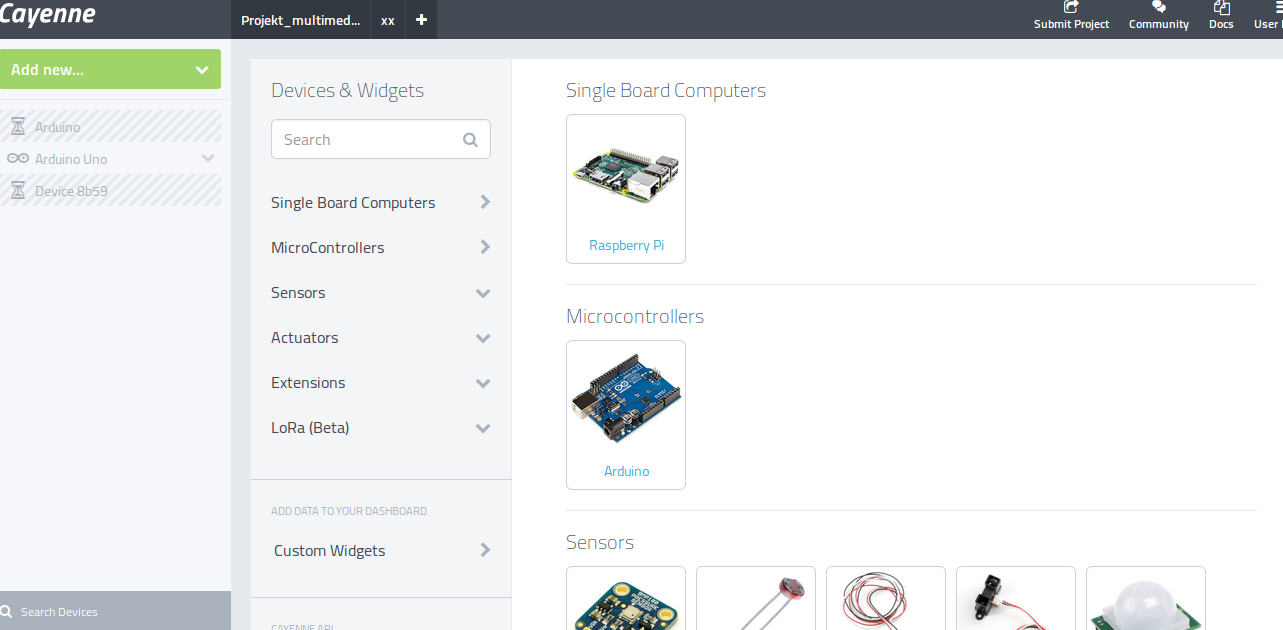
\includegraphics[width=\columnwidth]{images/7.png}
  \caption{Komponenty elektroniczne}
\end{figure}
Rysunek 8. przedstawia wybieranie zaimplementowanych już w środowisku Cayeene komponentów elektronicznych których chcemy użyć w projekcie. Znajdują się tu najpopularniejsze elementy jak czujnik temperatury DS18B20 i inne. Istnieje również wybór kontrolera naszego systemu może być to Arduino lub Raspberry PI.
\begin{figure}[!h]
  \centering
  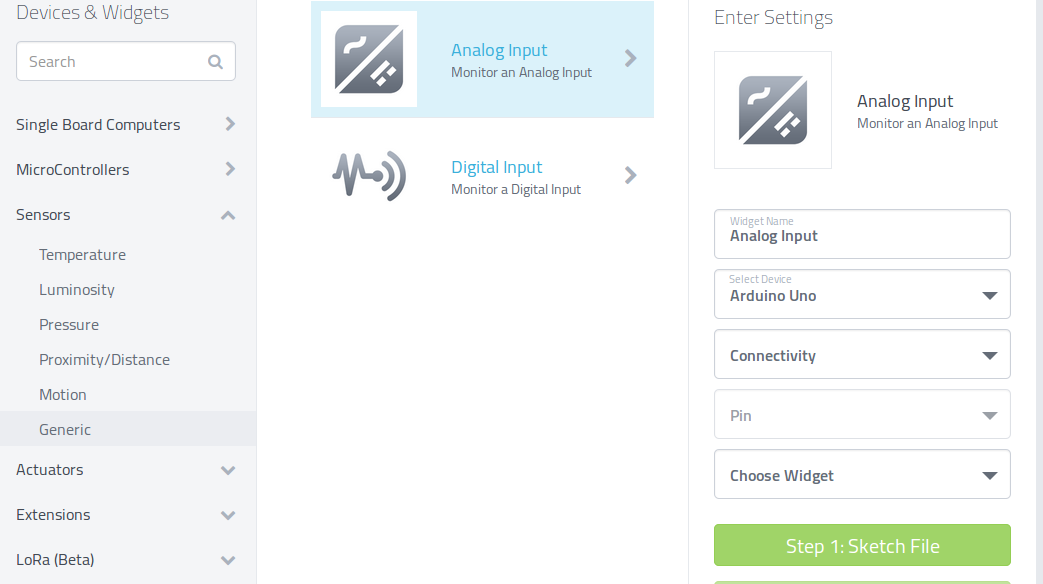
\includegraphics[width=\columnwidth]{images/8.png}
  \caption{Własne urządzenie}
\end{figure}

Rysunek 9. przedstawia dodawanie niezaimplementowanego w środowisku własnego urządzenia. Jak widać mamy dwa wejścia analogowe i cyfrowe które są używane do podpięcia urządzeń. Zauważyć można kontrolkę „Step1: Sketch File” po naciśnięciu jej wybierając zaimplementowane w środowisku urządzenia dostaniemy tekstowy opis połączenia, potrzebnych elementów jak rezystory czy kondensatory oraz tekstowy schemat połączenia urządzenia z naszym Arduino czy Raspberry PI.

\end{document}